\documentclass{article}

\usepackage[utf8]{inputenc}
\usepackage[english]{babel}

\usepackage{markdown}

\usepackage{amsmath}
\usepackage{hyperref}
\usepackage{url}
\usepackage{graphicx}
\usepackage{float}
\usepackage{multicol}
\usepackage[margin=2.5 cm]{geometry}
\usepackage{svg}

% Including dice package
%\usepackage{ttfdice-main/ttfdice}
%\usepackage{customdice/customdice}


\title{A Shelves Voyages}

\author{Nicholas Cornia, Orpheus Instituut}

\date{June 2025}

\begin{document}

\maketitle

\begin{multicols}{2}

\section*{What is this game about?}\label{whatisthisgameabout}

\textit{A Shelves Voyage} is a game about \textbf{discovery}, \textbf{plurality}, and \textbf{unexpected journeys} designed for researchers and librarians wishing to unchain the potential of knowledge graphs in their practice.

Furthermore, the game is suited for scholars willing to think in \textit{semantic triples}, a way to record information according to the Resource Description Framework (RDF) standard, exploring the possibilities of Linked Open Data in a ludic and playful manner.

During a game session, the players collaboratively build a small \textit{knowledge graph} by reconsidering their viewpoint on entities and concepts related to their research field, or the library catalogue of their institution. After each game session, a non-linear knowledge structure will emerge from the collaborative, and sometimes adversarial, effort of the player. This game encourages collaborative research between fellow researchers at any stage of their work, in opposition to solitary and competition-based inquiry.

We have introduced some randomness in the process to drive players outside their intellectual comfort zones, exploring the possibilities of unbeaten tracks and collaborative research.

An abstract currency, called "coins", will reflect the degree of selfishness of each player during the conversation. Participants are encouraged to balance their contribution by being generous with others and foster fruitful exchange of knowledge.

This game could be easily adapted for introductory talks, open discussions and panel sessions during conferences, and even brainstorming. Despite the scholarly theme given to the game, it could be played by any collective of people outside academia willing to explore conversation and decision making in a playful way.

\section{Game Mechanics}\label{gamemechanics}

To embrace the main objectives of this game, namely collaborative knowledge building and unexpected intellectual journeys, we have designed a series of game mechanics that will help the players emulate a fruitful and truly collaborative conversation.

\subsection{Entities and Statements}

\begin{figure}[H]
\centering
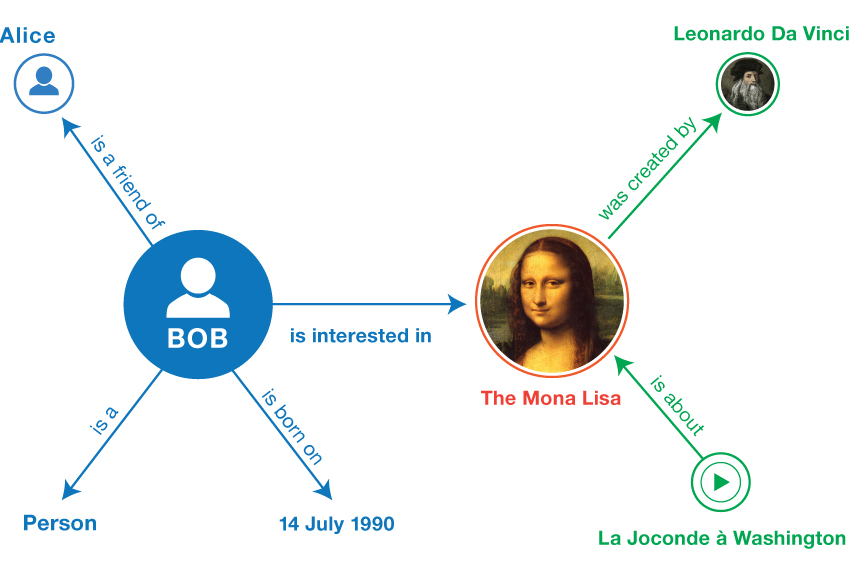
\includegraphics[scale=0.2]{figs/example-graph.jpg}
\caption{Example of knowledge graph. The nodes represents entities, while the directed edges and their labels imply statements.}
\end{figure}

A knowledge graph is a non-hierarchical data structure composed by entities, namely any sort of thing you can imagine, and statements connecting them.

A statement is represented by a semantic triple made of a subject, a predicate (or property) and an object. 

In \textit{A Shelves Voyages}, entities are represented by circular wooden disks that can store a small index card. Statements consist of two entities (wooden disks) connected by a colored cord with a post-it describing its predicate. For a visual example, see the figure above.

A meta-statement is a statement about a statement, providing additional information about it. A typical example of a meta-statement is a reference to a source that validates or describes the statement. Another example is an agent involved in the process. In game, represent this action by connecting the new entity to the cord representing the statement. For example, we can add "Wikipedia" to the statement "Mona Lisa was created by Leonardo da Vinci" by attaching a colored cord to the already existing cord between "Mona Lisa" and "Leonardo da Vinci".

\newpage

\subsection{Actions}

\textit{A Shelves Voyages} uses a pool of six-sided dice (d6s) to randomly determine the type of actions a player can perform during their turn. This game mechanics is widely used in modern board game design, allowing players to take actions after a process of input randomness. There are six actions, each one associated with a digit from 1 to 6.

\begin{enumerate}

\begin{figure}[H]
\centering

\includegraphics[scale=0.05]{figs/acorn.png}
\end{figure}

\item \textbf{Harvest}: choose one of the following options:
	\begin{itemize}
	\item Gain 2 coins.
	\item Draw a Minor Arcana card from the deck.
	\item Draw two Major Arcana cards and keep one.
	\end{itemize}
	
\begin{figure}[H]
\centering
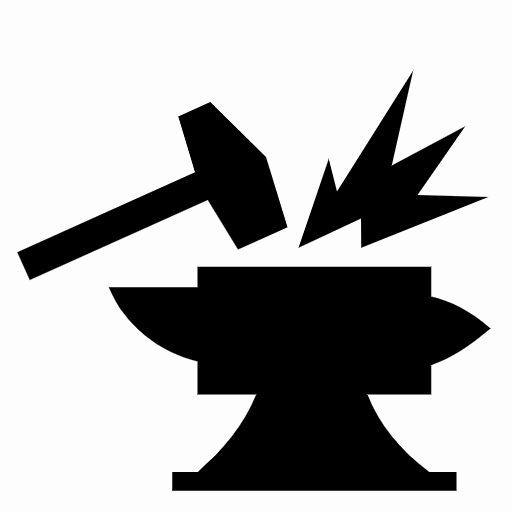
\includegraphics[scale=0.05]{figs/anvil-impact.png}
\end{figure}

\item \textbf{Co-Create}: Enhance the knowledge graph by 
\begin{itemize}
\item introducing a new entity and make a statement about it
\item connecting two elements on the knowledge graph
\item making a \textbf{meta-statement}, such as a reference to a source.
\end{itemize}
You have to \textbf{engage another player} in this process. This moment of shared agency can be stacked with the Resonance die mechanics.

\begin{figure}[H]
\centering

\includegraphics[scale=0.05]{figs/classical-knowledge.png}
\end{figure}

\item \textbf{Advocate}: Similar to the \textbf{Co-create} action, but you don't have to engage any player. \textbf{Gain 1 coin}.

\begin{figure}[H]
\centering

\includegraphics[scale=0.05]{figs/fox.png}
\end{figure}
   
\item \textbf{Manipulate}: Force another player to perform a Co-create, Advocate or Quarrel action about a topic chosen by you. \textbf{Give them 2 coins} and a \textbf{Manipulate token}. This token will be kept by the player until they fulfil their commitment.

\vspace{1cm} 

\begin{figure}[H]
\centering

\includegraphics[scale=0.05]{figs/crossed-sabres_w.png}
\end{figure}
   
\item \textbf{Quarrel}: Choose an entity and invite another player to discuss with you about it. At the end of the quarrel, the rest of the players can vote for the participant who provided the most convincing argument. The winner loses 2 coins, while the loser can immediately perform (without advancing their station in the Game of Goose) an Advocate action reflecting their argumentations. Both participants get a \textbf{Quarrel token}.

\begin{figure}[H]
\centering

\includegraphics[scale=0.05]{figs/spyglass.png}
\end{figure}
   
\item \textbf{Invent}: Perform any of the previous five actions at the cost of clearing your \textbf{Resonance pool}. If the pool is already empty, the player can perform the chosen action for free with no additional consequences.

\end{enumerate}

\subsection{Resonance system}

At the beginning of their turn, the active player rolls four six-sided dice (4d6) and looks for pairs of dice with the same value. They choose one pair and perform the corresponding action. For example, if the player rolls two 2 and two 5 they can decide to either perform the Create or the Quarrel action. The probability to at least get one pair of dice is about 72\% and the player can access dice from their and other players Resonance pools.

At the end of their turn, a player has to store an unused die into their Resonance pool, a bank of dice that can be used by all players at the table to increase the possibility to achieve a specific action. The following rules apply while using dice from Resonance pools:

\begin{itemize}
\item The active player can ask a die from another player's pool in exchange for sharing the action by determining together the entity and statement. Furthermore, the donor immediately earns 1 coin from the active player.
\item The active player can use a die from their own pool to construct a pair of dice in order to perform an action. If they choose so, they earn 1 coin from their pool.  
\end{itemize}

\subsection{Legacy}

Players can encourage the group to further digress about a certain entity on the knowledge graph by defining a Legacy. 

At the end of their turn, a player can ask the GM to place a meeple of their color to an entity in exchange for 2 coins. From that moment on, all players can perform actions involving that entity with the following advantages:

\begin{itemize}
\item A Quarrel provides a loss of 3 coins, instead of 2, for the winner while the looser performs their Advocate action without earning a coin.
\item  Invent actions only clear one die from your Resonance pool.
\item Using a die from your own Resonance pool does not let you earn a coin.
\end{itemize}


This mechanics is inspired by the collaborative storytelling game \textit{Microscope}\footnote{\url{https://lamemage.com/microscope/}}. 

\subsection{The Game of Goose}

Inspired by the board game \textit{Patchwork}, we decided to use a dynamic initiative system for our game as an alternative to the conventional clockwise or counter-clockwise turn order. Each player places a meeple on a Game of Goose board. At the end of each player's turn, their meeple will advance according to the performed action value. For example, if the player just performed the Manipulate action, they will advance their meeple four steps.

Usually, the player with meeple in the lowest station of the Game of Goose can take the next turn. In case of ties, the GM can choose which player goes first.

The GM has to decide beforehand which station will end the game. We advise the following values, but bear in mind that larger groups will take longer to reach the end station:

\begin{itemize}
\item 18 for a short session.
\item 32 for a comprehensive exploration.
\item 63 for a long session ranging multiple hours, for example a conference day.

\end{itemize}

\vspace{1cm}

\subsection{Tarot Cards}

Inspired by games with hidden objectives, such as \textit{Ticket to Ride}\footnote{\url{https://boardgamegeek.com/boardgame/9209/ticket-to-ride}}, and cards breaking up rules, we have introduced two special decks of cards.

In the classic tarot game, the first deck is composed of 22 Major Arcana cards while the second is made of Minor Arcana cards including four seeds of 14 cards each, 10 numerals and 4 figures. 

\subsubsection{Minor Arcana}

\begin{enumerate}
\item Treasure: Discard this card in exchange for 4 coins at any time. You can either increase or decrease your coins with this card.
\item Create: Perform the Create action without advancing your meeple's station at any time.
\item Advocate: Perform the Advocate action without advancing your meeple's station at any time.
\item Manipulate: Perform the Manipulate action without advancing your meeple's station at any time.
\item Quarrel: Perform the Perform action without advancing your meeple's station at any time.
\item Invent: Perform the Invent action without advancing your meeple's station at any time. You do not have to clear your Resonance pool.
\item Catalogue: You are allowed to use information from a catalogue or similar source of information, either digital or analog.
\item Medium: You are allowed to use an audio or visual object for one of your actions.
\item Turtle: Move a meeple backwards on the Game of Goose, either yours or owned by another player, for an amount of stations equal to the lowest result of 2d6.
\item Hare: Move a meeple forward on the Game of Goose, either yours or owned by another player, for an amount of stations equal to the highest result of 2d6.
\item Page: During another player's turn, you can force them to accept one die from your Resonance pool.
\item Knight: Reduce a maximum of 3 coins from another player and return them to the board.
\item Queen: During your turn, a player has to provide a die from their Resonance pool, without earning any coin.
\item King: Alter a Legacy on the knowledge graph by either removing it, change its position or ownership (colour).
\end{enumerate}

\subsubsection{Major Arcana}

Here is a list of interesting objectives for the players. Each of them tries to encourage unexpected behaviors and interesting emergent game-play.

\begin{enumerate}[I.]
% I
\item Reduce your Harmony score by half (rounded up) for each Legacy meeple you own on the knowledge graph.
% II
\item Divide your Harmony score by an amount equal to 2 times the length of the longest path you have created on the knowledge graph (rounded up). For example, if the maximal length of a path is 4, you will divide your Harmony score by 8, rounded up.
% III
\item Reduce your Harmony score by half (rounded up) for each disconnected component in the knowledge graph.
% IV
\item Exclude your Harmony score from the final result if the knowledge graph is fully connected, meaning that there is always a path connecting any given entity. In case of failure, double your Harmony score.
% V
\item Reduce your Harmony score by half (rounded up) for each meta-statement you created on the knowledge graph.
% VI
\item Exclude your Harmony score from the final result if no Manipulate tokens are left at the end of the game. In case of failure, double your Harmony score.
% VII
\item Reduce your Harmony score by half (rounded up) for each Quarrel token you own.
% VIII
\item Reduce your Harmony score by half (rounded up) for each Minor Arcana used or kept at the end of play.
% IX
\item Reduce your Harmony score by half (rounded up) for each Major Arcana in your hand after the first.
% X
\item Double your Harmony score for each die left in your Resonance pool. If there are no dice on your pool, exclude your Harmony score from your final result.
% XI
\item Reduce your Harmony score by half (rounded up) for each die left in the biggest Resonance pool of another player.
% XII
\item Divide your Harmony score by half (rounded up) if you have collected the least coins at the end of the game.
% XIII
\item Exclude your Harmony score from the final result if only one other player has collected an amount of coins lesser than yours at the end of the game. In case of failure, double your Harmony score.
% XIV
\item Divide your Harmony score by half (rounded up) if you have collected the most coins at the end of the game.
% XV
\item Exclude your Harmony score from the final result if only one other player has collected an amount of coins grater than yours at the end of the game. In case of failure, double your Harmony score.
% XVI
\item Reduce your Harmony score by half (rounded up) if your meeple is on the lowest station in the Game of Goose.
% XVII
\item Exclude your Harmony score from the final result if your meeple is on the penultimate station in the Game of Goose. In case of failure, double your Harmony score.
% XVIII
\item Reduce your Harmony score by half (rounded up) if your meeple is on the highest station in the Game of Goose.
% XIX
\item Exclude your Harmony score from the final result if your meeple is on the second highest station in the Game of Goose. In case of failure, double your Harmony score. In case of failure, double your Harmony score.
% XX
\item Reduce your Harmony score by half (rounded up) for each entity on the knowledge graph with only one statement associated to it.
% XXI
\item Divide your Harmony score by an amount equal to 2 times the maximal degree of an entity on the knowledge graph, where the degree is the number of statement involving the given entity.
% XXII
\item Reduce your Harmony score by half (rounded up) for each entity without any statement. This condition can only be achieved by entities introduced in the preparatory phase by the players. For example, if no player makes statements on 3 intial entities, then you will divide your Harmony score by 6 (rounded up).
\end{enumerate}

\subsection{Harmony score}

\textit{A Shelves Voyages} is a cooperative game that takes inspiration to games such as \textit{Hanabi}\footnote{\url{https://boardgamegeek.com/boardgame/98778/hanabi}} and \textit{Tales of Kunugi}\footnote{\url{https://boardgamegeek.com/boardgame/422620/tales-of-kunugi}}, where players work together while sharing partial information about the game-world. This hidden knowledge is encoded in the Major Arcana cards, objectives that cannot be shared by the players, providing unexpected result in the final amount of coins a player collects at the end of the game.

The main goal of the group is to achieve the lowest collective Harmony score, reflecting balance and collaboration between the players during the creation of the knowledge graph.

When a player reaches the designated end-of-game station, the game session ends.  The GM computes the average value (rounded up) for all players, based on the amount of coins they own. 

Afterwards, each player computes the absolute distance between their coin amount and the aforementioned average value. This number is called the Harmony score of a player. On this stage, each player reveals their Major Arcana cards and adjusts their Harmony score according to the achieved objectives. Finally, the GM computes the sum of all the Harmony scores, and the final result will reflect how balance and collaborative the game session has been.

For example, a session with 5 players ends with coins amounts of 8, 12, 10, 22 and 14.
The average value is 14 (rounded up) and for each player we have Harmony scores of 6, 2, 4, 8, 0. At this moment, players reveal their Major Arcana cards that will alter their Harmony scores to 1, 4, 2, 0, 0 The final average Harmony score for the group is 7.

Here an Average Harmony score heuristic table, based on the number of players $n$:

\begin{table}[H]
    \centering
    \begin{tabular}{|l|l|}
    \hline
        Average Harmony score range & victory level \\ \hline
        0 to $n$ & Excellent \\ \hline
        $n+1$ to $2n$ & Great \\ \hline
        $2n+1$ to $3n$ & Good \\ \hline
        $3n+1$ to $4n$ & Mediocre \\ \hline
        more than $4n+1$ & Unbalanced \\ \hline
    \end{tabular}
\end{table}

%\newpage

\section{Playing the game}

\subsection{Game Master}

Before the start of the session, the players designate one of them as Game Master. They act as moderators and final judge for the session. Such person should be familiar with the rules and being comfortable in taking decisions and monitor the behaviour of each participant, encouraging a playful and respectful environment.

\subsection{Set-up}

For this game you will need:

\begin{itemize}
\item 3-10 players, including a GM.
\item 1 to 6 hours, depending on the size of the group and the end-of-game station designated.
\item Pencils, post-its and small index cards.
\item Coloured cords and meeples.
\item 8 six-sided dice per player.
\item Movable flat surfaces to store index cards. We use circular wooden disks with a series of holes on their boundaries.
\end{itemize}

\subsection{Preparatory phase}

Each player collects 4 initial coins, 4 six-sided dice and draws a Major Arcana card from the deck.

Afterwards, the GM asks each player to place one entity on the board, without adding any statement to it. These entities can be tied to a theme, such as the players' research interest or topics of a conference.

Once every player has placed an entity on the board they define their initial position on the Game of Goose by rolling a d6 and place their meeple on the station correspondent with the die result. Ties will eventually emerge, and the GM has the responsibility to decide which player goes first.

Finally, the group determine the end-of-game station that will trigger the end of the session.

\subsection{Player's turn}

\begin{enumerate}
\item Roll 4d6 and look for matching pairs of digits.
\item Add one die from your own Resonance pool or ask it from another player.
\item Choose one pair of dice and perform the corresponding action.
\item Gather or pay coins.
\item Store one unused die from the initial 4d6 and add it to your Resonance pool
\item Increase your station on the Game of Goose according to the action value.
\end{enumerate}

\subsection{Game session}

The active player is the one with meeple at the lowest station of the Game of Goose. In case of ties, the GM decides which player goes first.

Players are free to use at any times Minor Arcana cards, and place Legacy tokens on board.

\subsection{End of game}

Once a player reaches the end-of-game station the session is over.

\begin{itemize}
\item Each player calculates their final amount of coins.
\item The GM computes the average value of those amounts.
\item Each player calculates their Harmony score, the absolute distance between their amount of coins and the average value.
\item Each player alters their Harmony score according to the objectives on their Major Arcana cards.
\item The sum of all Harmony scores is the final result.
\end{itemize}

\section{Advice}

\subsection{Modular rule-set}

In order to make the game accessible to a wider audience, not necessarily comfortable playing board games, we have tried to construct our rule-set in a modular way, allowing GMs to neglect some aspect of the game-mechanics for new players.

\begin{itemize}
\item Minor and Major Arcana bring end-of-game objectives and extra randomness in the game session and can be excluded without any further modification. In that case, the Harvest action will only provide 2 coins.
\item The Game of Goose can be neglected in favour of a more classical clockwise turn-based initiative or a full free-form "popcorn" initiative. Be aware that some actions require more time at the table than others. Make sure to remove all Major Arcana cards related to this mechanics.
\item Legacy tokens are also optional. Make sure to remove all Major Arcana cards related to this mechanics.
\end{itemize}


\end{multicols}

\end{document}
